\chapter{Fundamentação das Máquinas de vetores de suporte} \label{cap:svm}

As Máquinas de Vetores de Suporte (SVM, do inglês \textit{Support Vector Machine}) surgiram com o emprego da teoria da aprendizagem estatística, desenvolvida pelo pesquisador Vladimir Vapnik e colaboradores \cite{Vapnik1998}. Mais precisamente, a SVM é uma implementação do método de minimização estrutural de risco. Este método busca minimizar o erro do conjunto de treinamento, juntamente com o erro do conjunto de teste. O objetivo da SVM é criar um bom meio de aprendizagem que separe grandes dimensões através de um hiperplano, de tal maneira que as margens sejam ótimas, que seja computacionalmente eficiente e capaz de lidar com amostras de tamanhos da ordem de 100 000. Nesta Capitulo será revisada a teoria básica para a construção da SVM. Na Seção \ref{S1}, a SVM será introduzida como parte do conjunto de métodos de aprendizagem dentro das redes neurais, serão apresentados os princípios básicos de redes neurais necessários, para a compreensão deste capitulo. Na Seção \ref{S2}, vamos ver os paradigmas de aprendizagem e situaremos a condição da SVM ante a estes paradigmas. Em seguida veremos na Seção \ref{S3} a teoria que originou a criação da SVM. Na sequência será revisado na Seção \ref{Teot}, conceitos de otimização necessários para a solução da SVM. E por fim será visto a teoria da SVM primeiramente para os casos onde os dados são linearmente separáveis Seção \ref{cap:svm:svm-l}. Então para os casos onde os dados não separados linearmente Seção \ref{cap:svm:svm-nl}. Finalizando o capitulo com os métodos utilizados para a solução da SVM Seção \ref{spq}.

\section{Introdução as Redes Neurais Artificiais} \label{S1}
As Redes Neurais Artificiais (RNA do inglês \textit{Artificial Neural Networks}) foram motivadas a partir funcionamento do  cérebro, este é um complexo sistema constituído de aproximadamente duzentos bilhões de células que pode computar problemas com características não triviais, como computações em paralelo, ou problemas não lineares. A estrutura do cérebro é organizada em subunidades chamadas de neurônios, que são responsáveis pelos cálculos realizados no cérebro \cite{Haykin99}.

Os neurônios se interligam a fim de realizar tarefas como: o reconhecimento de padrões; percepção; e coordenação motora. Eles têm a capacidade de adaptar-se ao ambiente, através de estímulos enviados para eles. A Figura \ref{fig:neuronio-nat} apresenta um neurônio natural.

\begin{figure}[htb]
	\centering
	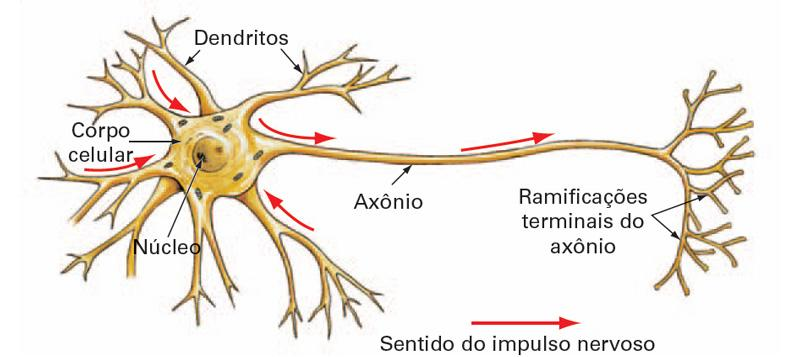
\includegraphics[scale=0.5]{./figuras/neuronio-nat.jpg}
	\caption{Neurônio natural}
	\label{fig:neuronio-nat}
\end{figure}

Com base no comportamento dos neurônios biológicos, pesquisadores modelaram matematicamente o neurônio. Um neurônio é uma unidade de processamento fundamental em uma RNA. A representação dele em forma de diagramas pode ser vista na Figura \ref{fig:neuronio_artificial}.

\begin{figure}[htb]
	\centering
	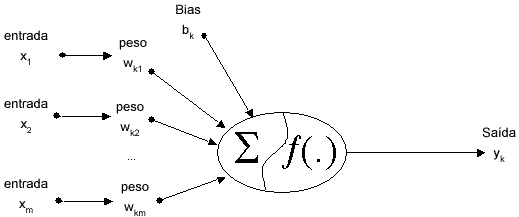
\includegraphics[scale=0.8]{./figuras/neuronio_artificial.jpg}
	\caption{Neurônio artificial (Adaptado de \cite{Haykin99})}
	\label{fig:neuronio_artificial}
	%http://www.lncc.br/~labinfo/tutorialRN/frm1_neuronio.htm
\end{figure}

Podemos observar pela figura um conjunto de ligações sinápticas e seus respectivos pesos $w$, este é um vetor, ligando os dados do também vetor de entrada $x$ ao somador e $m$ é o numero de dados. É realizado o produto entre os vetores $x$ e $w$ e o resultado é aplicado ao somador. A soma de todas as entradas é processada por uma função de saída $f(.)$, também conhecida como função de ativação, que limita a amplitude de saída de um neurônio. As funções de saída mais comuns são: função limiar; função sigmóide; e função hiperbólica. A função Limiar apresentada na Equação \ref{svm:E0} merece atenção devido ela ser adequada às SVMs.

\begin{equation} \label{svm:E0}
y = \left\{\begin{matrix}
+1, & se\ F & \left( \sum_{i=0}^{m=1} x_{i}w_{i} + b \right) > 0 \\ 
														       \\		
-1, & se\ F & \left( \sum_{i=0}^{m=1} x_{i}w_{i} + b \right) < 0
\end{matrix}\right.
\end{equation}

O parâmetro externo $b$ é denominado bias, ele aumenta ou diminui o número de grau de liberdade no modelo, o que permite a rede uma capacidade maior de se ajustar.

Existem diversos algoritmos baseados no modelo de neurônio apresentado, como o Perceptron, Perceptrons de Múltiplas Camadas, e as SVMs. A combinação dos neurônios nas SVMs é mostrada na Figura \ref{fig:SVM-RNA}. O SVM é uma RNA com duas camadas, na camada de saída há apenas um neurônio que é responsável pela construção da função linear no espaço.

\begin{figure}[htb]
	\centering
	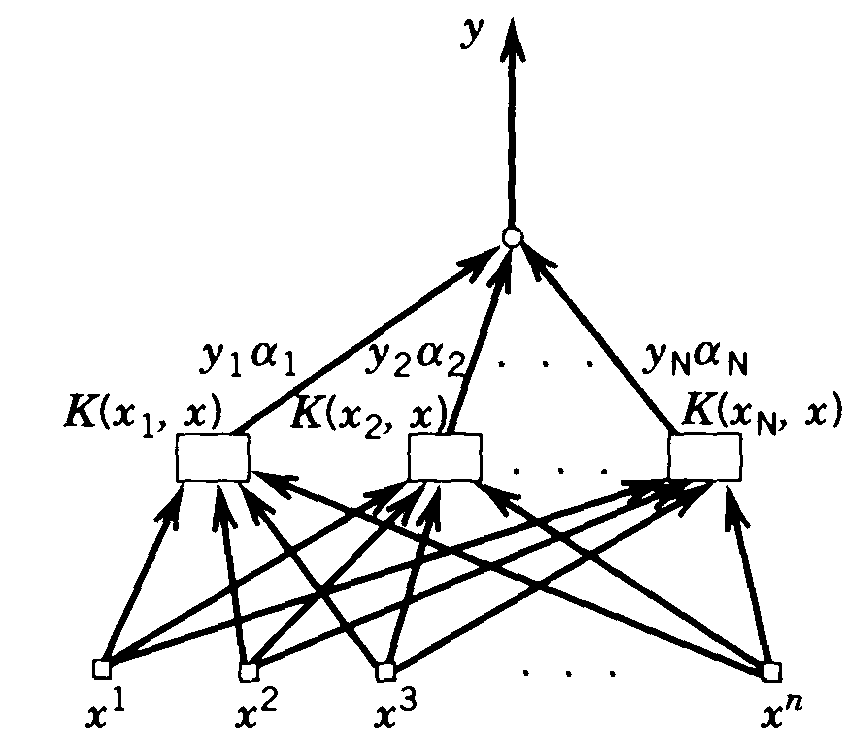
\includegraphics[scale=0.5]{./figuras/SVM-RNA.png}
	\caption{Representação da rede de neurônios do SVM \cite{Vapnik1998}}
	\label{fig:SVM-RNA}
\end{figure}

\section{Conceitos básico de aprendizagem } \label{S2}

A aprendizagem de máquina (AM) é o processo no qual algoritmos desenvolvidos para o computador são capazes de obter conhecimento sobre um determinado problema a partir de resultados observados numa parte desse problema, e gradativamente melhorar o desempenho da aprendizagem. O sistema de aprendizagem é estimulado por um ambiente, este estímulo resulta em modificações em sua estrutura interna e por fim na maneira que o sistema vai responder ao ambiente. As técnicas desenvolvidas para a AM tem como princípio a inferência indutiva. A inferência indutiva para aprendizagem pode ser dividida em três grupos: aprendizagem supervisionada (com professor), aprendizagem por reforço (sem professor)  e aprendizagem não-supervisionada (sem professor).

Na aprendizagem supervisionada temos a figura de um professor, que é um individuo com conhecimentos sobre o ambiente e consequentemente dos exemplos de entrada do sistema de aprendizagem, este conhecimento é na forma: entrada e saída desejada. Este tipo de representação é comumente conhecido como entrada rotulada. O processo da aprendizagem supervisionada consiste primeiramente na etapa de treinamento da máquina de aprendizagem, onde o professor ensina o sistema com o conjunto de exemplos rotulados, o sistema a cada iteração ajusta sua saída conforme a saída esperada, para que a saída seja cada vez mais próxima da saída desejada, com isto o algoritmo de aprendizagem extrai a representação do conhecimento. Então a partir dessa representação, novos exemplos que não foram apresentados anteriormente, quando apresentados, espera-se que tenham suas saídas produzidas corretamente.

A aprendizagem por reforço diferente da aprendizagem supervisionada não utiliza o auxílio de um professor e de exemplos rotulados. Neste tipo de aprendizagem há uma interação contínua com o ambiente, com o objetivo de melhorar o desempenho. O agente (p. ex. robô) observa o estado do ambiente então toma uma decisão. A cada ação tomada os resultados podem ser positivos ou negativos e esses processos são memorizados, a máquina de aprendizagem tem por função descobrir quais são as melhores ações a serem tomadas e realimentar o ambiente.

Na aprendizagem não-supervisionada, assim como na aprendizagem por reforço, não utiliza-se o auxílio de um professor e exemplos rotulados. A máquina de aprendizagem aprende a representar as estradas conforme uma medida de qualidade. Os parâmetros da estrutura interna da máquina são otimizados segundo esta medida. Uma vez que as regularidades estatísticas dos dados estejam ajustadas, a máquina pode formar representações internas para codificar as características de entrada e criar automaticamente novas classes \cite{Haykin99}.

Neste trabalho será dada atenção a aprendizagem supervisionada, em específico na técnica de aprendizagem de SVM. Os conjuntos de exemplos rotulados serão da forma $(x_{i},y_{i})$, onde $i$ vai de $1,2,...,m$ e cada $x_{i}$ representa um dado, ao longo do texto também será referenciado $x_{i}$ como pontos ou exemplos de treinamento, e $y_{i}$ representa o rótulo de um dado. O objetivo é produzir um classificador que separa os dados em diferentes classes conforme os seus rótulos, este processo também é conhecido como treinamento, e então prever a classe de novos exemplos que não estão contidos no conjunto de treinamento.

Os valores assumidos nos rótulos neste trabalho são discretos $1,2,...,k$, que caracteriza um problema de classificação, caso os valores sejam contínuos o problema é de regressão. Quando assumimos um valor de $k=2$, restringimos nosso problema para uma classificação binária, para $k > 2$ o problema se torna em um de multi-classificação, aqui será tratado apenas problemas de classificação binária.

A figura \ref{fig:classificador_supervisionado} apresenta uma simplificação da forma de representação de um classificador em aprendizado supervisionado.

\begin{figure}[htb]
	\centering
	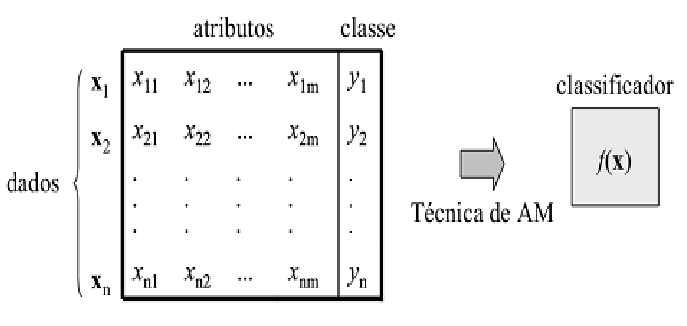
\includegraphics[scale=0.5]{./figuras/classificador_supervisionado.png}
	\caption{Classificador de aprendizagem supervisionado \cite{Lorena2007}}
	\label{fig:classificador_supervisionado}
\end{figure}


\section{Teoria do aprendizado estatístico}\label{S3}

A teoria do aprendizado estatístico (TAE) estuda as propriedades matemáticas das máquinas de aprendizagem. Estes estudos auxiliam na escolha e projeção, de uma função (ou classificador) $f$ a partir dos dados de treinamento $\tau$, tal que $f$ seja ótima. Para a escolha são utilizadas as propriedades matemáticas, que levam em conta o desempenho (p. ex. quão rápido o algoritmo converge) no conjunto de dados e a complexidade. Com isto é possível ter uma estimativa do desempenho para novos conjuntos de dados.


\begin{figure}[htb]
	\centering
	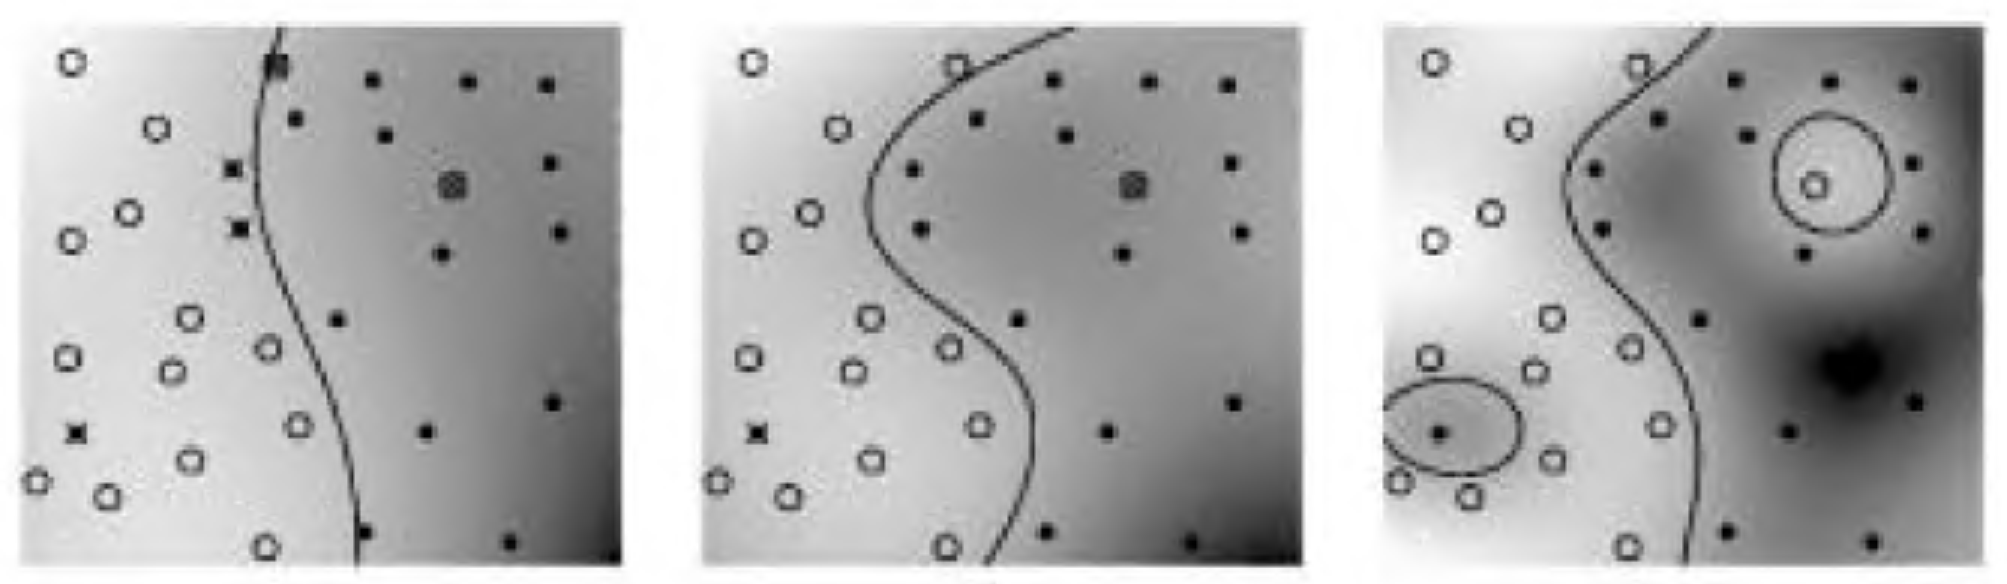
\includegraphics[scale=0.3]{./figuras/2dtoyexample.png}
	\caption{Três modelos para a classificação binaria de dados \cite{Scholkopf2002}}
	\label{fig:2dtoyexample}
\end{figure}

No exemplo dado por \cite{Scholkopf2002}, a tarefa é separar os pontos sólidos em negrito que assumem o valor 1 dos círculos que assumem o valor -1, mostrado na Figura \ref{fig:2dtoyexample}. 

No gráfico mais a direita, a função de classificação separa corretamente todos os dados, inclusive dois \textit{outliers} \footnote{Outliers são dados classificados incorretamente, tais dados invadem o espaço da classe oposta a dele.}. Porém para dados de teste é grande a probabilidade dela gerar um erro, devido a sua grande especificidade. Este tipo de caso é chamado de superajustamento do modelo aos dados de treinamento, comumente conhecido pelo termo em inglês \textit{overfitting}. Para evitar o superajustamento podemos tentar um modelo mais simples como o gráfico mais a esquerda, que tem uma função de classificação praticamente linear. Entretanto esta separação não somente desclassifica os \textit{outliers} mas também casos considerados simples. Temos assim um sub-ajustamento, porque o classificador não é capaz de ajustar até mesmo aos exemplos de treinamento. Por último, o gráfico central que tem uma complexidade intermediária e consegue classificar a maioria dos pontos corretamente.

Os dados usados na escolha do classificador são gerados de uma probabilidade de distribuição $P(x,y)$ desconhecida , tal que $f$ classifique dados que não fazem parte do conjunto de treinamento corretamente. Dados gerados dessa forma é comumente conhecidos como independente e identicamente distribuídos (\textit{iid}). 

A melhor função $f$ é a que tem o cálculo do erro esperado, ou risco, minimizado para os dados de teste. Na Equação \ref{TA:E1}, $c(f(x),y)$ é a função de ativação relacionando a previsão $f(x)$ com a saída desejada $y$. Neste caso a função de ativação é assumida como $c(f(x),y) = \frac{1}{2} \mid y - f(x) \mid$. O valor da função é definido pela Equação \ref{funcx} de acordo com \cite{Burges1998Support, Scholkopf2002}.

\begin{equation} \label{funcx}
c(f(x),y) = \left\{\begin{matrix}
0, & se\ x \text{ é classificado corretamente} \\ 
														       \\		
1, & se\ x \text{ é classificado incorretamente}
\end{matrix}\right.
\end{equation}

\begin{equation} \label{TA:E1}
R(f) = \int c(f(x),y)dP(x,y)
\end{equation}

Infelizmente o risco não pode ser minimizado diretamente, uma vez que a distribuição de probabilidade $P(x,y)$ é desconhecida. Então utilizamos o processo de minimização do risco empírico de $f$ (Equação \ref{TA:E2}), que mede o desempenho do classificador nos dados de treinamento, por meio da taxa de classificações incorretas obtidas \cite{Muller2001}.

\begin{equation} \label{TA:E2}
R_{emp}(f) = \frac{1}{n} \sum_{i=1}^n c(f(x_{i}),y_{i})
\end{equation}

É possível dar condições para a máquina de aprendizagem, a qual assegura que assintoticamente (com $n \rightarrow \infty$) o risco empírico irá convergir para o risco esperado \cite{Muller2001}. Em outras palavras, permitindo que $f$ seja escolhida a partir de um conjunto de funções $F$ é sempre possível encontrar uma $f$ com pequeno risco empírico. Entretanto para pequenas amostras pode ocorrer o superajustamento. Então um menor erro não pode ser obtido apenas minimizando o erro de treinamento. Para evitar este tipo de problema deve-se restringir a classe de funções da qual $f$ é extraída \cite{Scholkopf2002}. Para isto existem diversas abordagens, e cabe a TAE apresentar quais conjuntos tem capacidade apropriada para a quantidade de dados de treinamento para a função $f$. Esta teoria também provê limites no risco esperado de uma função de classificação, que podem ser empregados na escolha do classificador.

Um outro limite importante da TAE é o limite de risco limitado. Este relaciona o risco esperado de uma função ao seu risco empírico e a um termo de capacidade. A Equação \ref{TA:E3} apresenta o risco limitado.

\begin{equation} \label{TA:E3}
R(f)\leq R_{emp}(f)+\sqrt{\frac{h\left(ln(\frac{2n}{n})+1\right) - ln (\frac{\theta}{4})}{n}}
\end{equation}

Onde, $h$ é a dimensão Vapinik-Chevonenkis (VC) da classe de funções $F$ que $f$ pertence, o limite da Equação \ref{TA:E3} é garantido com probabilidade de $1 - \theta$, em que $\theta \in [0,1]$, $n$ representa a quantidade de dados de treinamento, e todos os elementos que estão na raiz fazem parte do termo de capacidade.

É possível fazer algumas observações no risco limitado. A primeira, é que ele é independente de $P(x,y)$, e a segunda, é que nem sempre é possível calcular o lado esquerdo da equação, porque ele depende de $P(x,y)$. Por último, se $h$ for conhecido, possibilita facilmente calcular o lado direito da equação, e escolhendo um $\theta$ pequeno, isto é escolhendo a máquina que minimiza o lado direito, estamos escolhendo a máquina com menor limite superior no risco atual \cite{Burges1998Support}.

A dimensão VC separa os dados através de uma função em um certo modo que possibilita atribuir rótulos nos dados. Como os rótulos são binários, a quantidade máxima de rótulos diferentes para $m$ dados é $2^m$. Uma função "boa"\  é capaz de realizar $2^m$ separações, neste caso é dito quebrar os $m$ pontos. A dimensão VC é definida como o maior $m$ que existe em um conjunto de $m$ pontos, que são separados pela função, e $\infty$ caso $m$ não exista \cite{Scholkopf2002}.

A Figura \ref{fig:vc-dimensionexample} mostra um exemplo de VC. Existe $2^3=8$ caminhos de separar os 3 pontos em duas classes. Os dados podem ser separados por hiperplanos e a função de classe pode quebrar 3 pontos.

\begin{figure}[htb]
	\centering
	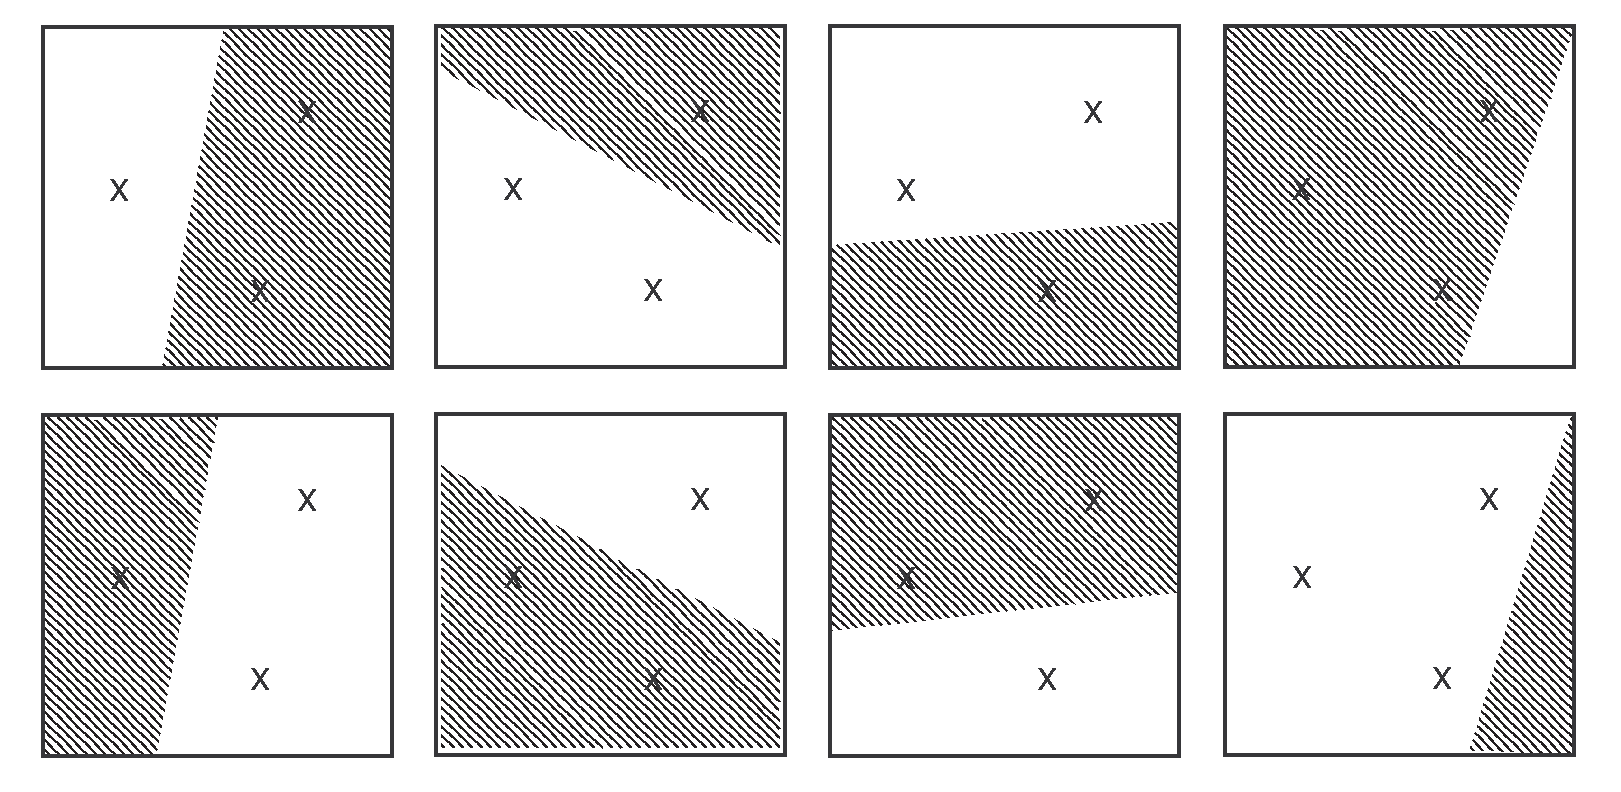
\includegraphics[scale=0.3]{./figuras/vc-dimensionexample.png}
	\caption{Exemplo de dimensão VC \cite{Scholkopf2002}}
	\label{fig:vc-dimensionexample}
\end{figure}


\section{Teoria da otimização} \label{Teot}

A teoria da otimização está relacionada no desenvolvimento da técnica do SVM, em especial em casos em que a função de custo é uma função quadrática convexa, com restrições que são lineares. Estes tipos de problemas são chamados de problemas quadráticos. O estudo destes problemas é importante, porque ele provê algoritmos e define condições para a resolução de problemas com características às da SVM \cite{Cristianini2000}. Nesta seção será apresentada de forma simplificada os problemas quadráticos \label{Teot:S1}. % falar de lagrange e dualidade

\subsection{Problema quadrático} \label{Teot:S1}

O problema quadrático na forma primal é definido da seguinte maneira:

\begin{equation} \label{Teot:E1}
\text{Minimizar}\  f(w),\ w \in \Omega
\end{equation}

\begin{equation} \label{Teot:E2}
\begin{matrix}
\text{Sujeito às restrições: } & g_{i}(w) \leq 0,\ i=1,...,k, \\ 
&    h_{i}(w) = 0,\ i=1,...,m  
\end{matrix}
\end{equation}

Onde as funções $f,\ g_{i},\ i=1,...,k, $ e $h_{i},\ i=1,...,m$ definidas no domínio $\Omega \subseteq \Re^n$, $f(w)$ é a função objetivo, $g_{i}(w)$ é a restrição de desigualdade  e $h_{i}(w)$ é a restrição de igualdade.

Uma função $f(w)$ é definida como convexa para $w \in \Re^n$ se $\forall w, u \in \Re^n$ e para qualquer $\theta \in (0,1)$, tem-se:

\begin{equation} \label{Teot:E3}
f(\theta w + (1 - \theta)u) \leq \theta f(w) + (1 - \theta)f(u).
\end{equation} 

Uma função convexa em um problema de minimização sempre possui uma solução global, o que se torna uma vantagem no tratamento do problemas quando a função é convexa \cite{Cristianini2000}. O teorema de Minimização Convexa, assegura essa propriedade onde: um conjunto convexo $D \subset \Re^n$ e $f:D \rightarrow \Re$ uma função convexa em $D$. Então todo o minimizador local da função $f(x)$ em $x \in D$ é global \cite{Ales2008}.

\subsection{Teoria do Lagrangeano}\label{Teot:S2}

Esta teoria foi desenvolvida por Lagrange em 1797, que generalizava um resultado de Fermat de 1629, posteriormente em 1951 foi estendida por Kuhn e Tucker. A junção destes avanços provê eficientes soluções para a tarefa de otimização de SVMs.

\textbf{Teorema de Fermat} A condição necessária para que $w^*$ seja mínimo de $f(w), f \in C^1$, é:

\begin{equation} \label{Teot:E4}
\frac{\partial f(w^*)}{\partial w} = 0
\end{equation}

Desde que $f$ seja um função convexa, essa condição é o suficiente. Em resumo, se $f \in C^1$, basta encontrar o ponto com a derivada primeira igual à zero, que será encontrado o mínimo da função.

Precisamente, um Lagrangiano é definido como a função objetivo somado a combinação linear das restrições, onde os coeficientes de combinação são chamados de multiplicadores de Lagrange \cite{Cristianini2000}. 

Dado um problema de otimização com função objetivo $f(w)$, e restrições de igualdade $h_{i}(w) = 0, i=1,...,m$, a função Lagrangiana é definida como:

\begin{equation}\label{Teot:E5}
L(w,\alpha) = f(w) + \sum_{i=1}^m \alpha_{i} h_{i}(w)
\end{equation}

Onde os coeficientes $\alpha_{i}$ são os multiplicadores de Lagrange.

\textbf{Teorema de Lagrange} Uma condição necessária para um ponto $w^*$ ser mínimo da função $f(w)$ sujeito a $h_{i}(w) = 0, i-1,...,m$ com $f,h_{i} \in C^1$, é:

\begin{equation} \label{Teot:E6}
\begin{matrix}
\frac{\partial L(w^*, \alpha^*)}{\partial w}  = 0 \\ \\
\frac{\partial L(w^*, \alpha^*)}{\partial \alpha} = 0
\end{matrix}
\end{equation}

para algum valor de $\alpha^*$. Isto prova que $L(w,\alpha^*)$ é uma função convexa de $w$.

A definição generalizada da função Lagrangeana, onde o problema de otimização contém as restrições de igualdade e desigualdade é: dados o problema de otimização \ref{Teot:E2} e o domínio $\Omega \subseteq \Re^n$ defini-se a função Lagrangeana Generalizada com mostrado na Equação \ref{Teot:E7}.

\begin{equation}\label{Teot:E7}
L(w,\alpha,\beta) = f(w) + \sum_{i=1}^k \beta_{i}g_{i}(w)+\sum_{i=1}^m \alpha_{i}h_{i}(w) = f(w)+\beta ' g(w)+\alpha ' h(w)
\end{equation}

O próximo passo é definir Lagrange na forma de problema dual. O problema dual é associado ao problema original (primal) facilitando a resolução do problema.

O problema dual Langrangeano pode ser definido como: dado um problema na forma primal \ref{Teot:E2}, com $\Omega \in \Re^n$, o problema dual é dado pela Equação \ref{Teot:E8}.

\begin{equation} \label{Teot:E8}
\begin{matrix}
\text{Maximizar} & \theta(\alpha,\beta) \\ 
\text{Sujeito as restrições}&    \alpha \geq 0
\end{matrix}
\end{equation}

onde: $\theta(\alpha,\beta) = inf_{w \in \Omega}L(w,\alpha,\beta)$

Uma importante definição que surge é o \textit{Gap} Dual. \textit{Gap} é a diferença entre os valores da função objetivo do modelo primal e do modelo dual \cite{Cristianini2000}. O \textit{gap} está relacionado com a solução ótima encontrada quando o valor da função objetivo primal $w$ é igual à função objetivo dual $\theta$, quanto mais próximo de zero estiver o \textit{gap} dual, mais próximo está da solução ótima do problema.

O teorema forte da dualidade afirma o que foi mencionado no parágrafo anterior, onde dado um problema de otimização \ref{Teot:E2}, com $\Omega \in \Re^n$, onde $g_{i},h_{i}$ são funções afins, o \textit{gap} dual é zero. Isto garante que os problemas dual e primal tenham o mesmo valor para problemas de otimização \cite{Cristianini2000}.

A solução ótima para um problema otimização generalizado, é condicionada ao teorema de Kuhn-Tucker. Onde, dado um problema de otimização \ref{Teot:E2}, com $\Omega \in \Re^n$, com $f \in C^1$ e $g_{i},h_{i}$ com funções afins, as condições necessárias e suficientes para que $w^*$ seja ótimo são a existência de $\alpha^*,\beta^*$, tais que:

\begin{equation}
\begin{matrix}
\frac{\partial L(w^*,\alpha^*,\beta^*)}{\partial w} = 0 \\ 
\frac{\partial L(w^*,\alpha^*,\beta^*)}{\partial \alpha} = 0 \\ 
\beta_{i}g_{i}(w^*) = 0 \\
g_{i}(w^*) \leq 0 \\
\beta^* \geq 0, i=1,...,k.
\end{matrix}
\end{equation}

%O resulta acima mostra que a definição de Multiplicador de Lagrange é uma extensão da noção do multiplicador na condição  de Karush-Kuhn-Tucker \cite{Cristianini2000}.

Toda a teoria estudada é fundamental para o entendimento teórico da SVM, uma vez que a SVM envolve a minimização de um problema quadrático convexo.

\section{SVMs lineares}\label{cap:svm:svm-l}

A teoria da SVM está fortemente ligada com a teoria da dimensão VC, uma vez que, na SVM é feito uma separação dos dados através de um hiperplano. A dimensão VC pode ser limitada pela margem: rígida ou suave. A diferença entre os dois grupos é que os classificadores SVM de margem rígida não permitem ruídos e \textit{outliers} nos dados, já a margem suave é uma extensão mais relaxada da SVM com margem rígida, permitindo tais tipos de dados. Primeiramente será abordado a SVM com margem rígida, que é um caso mais simples com fins didáticos. Para problemas práticos a SVM com margens suave é mais apropriada, esta será abordada na sequência.

\subsection{SVM com margem rígida} \label{svmL:S1}

Assume-se um conjunto de treinamento de dados $T$ com $n$ dados formado pelo par de dados $(x_{i},y_{i})$ onde $x_{i} (i = 1,....,n ), x_{i} \in R^{d}, d = 1,2,...,d $  são os dados de treinamento e $y_{i} (i = 1,....,n), y_{i} \in {-1,+1}$ são os respectivos rótulos de $x_{i}$. Os rótulos $y_{i}$ assumem dois possíveis valores $+1$ para dados da classe 1 e $-1$ para dados da classe 2. Se estes dados são linearmente separáveis, existe uma superfície de decisão que separa os dados positivos (+1) dos negativos (-1). A equação da superfície de decisão na forma de um hiperplano separador é apresentada na Equação \ref{svm:hp-sep}, onde $w\cdot x$ é o produto escalar entre os vetores $w$ e $x$, $w$ é um vetor de pesos ajustável, e $w \in R^{d}$, portanto $w$ também faz parte do conjunto de entradas (ou dados de treinamento), $b \in R$ é um bias. Os pontos $x$ que se encontram no hiperplano satisfazem $w\cdot x + b = 0$, onde $w$ é perpendicular ao hiperplano e $ \frac{b}{\parallel w \parallel}$ é a distância perpendicular do hiperplano até a origem \cite{Burges1998Support}.
%A menor distância distancia do dado mais próximo do hiperplano separador é chamado de $d_{+}$ para dados positivos ou $d_{-}$ para dados negativos. Uma margem de um hiperplano separador é a soma das distâncias positivas e negativas($d_{+}+d_{-}$) 

\begin{equation} \label{svm:hp-sep}
	f(x) = w\cdot x + b = 0
\end{equation}

Multiplicando $w$ e $b$ pela mesma constante é possível obter infinitos hiperplanos equivalentes. Um hiperplano é definido na forma canonical, se $w$ e $b$ são escalados de tal forma que os dados mais próximos do hiperplano $w\cdot x + b = 0$ satisfaça a Equação \ref{svm:E2} \cite{Scholkopf2002}:

\begin{equation} \label{svm:E2}
	\mid w\cdot x_{i} + b\mid = 1
\end{equation}
 
Essa forma implica na inequação \ref{svm:E3}.
\begin{equation} \label{svm:E3}
\left\{\begin{matrix}
w \cdot x_{i}+b \geq + 1 & para & y_{i} = +1 \\ 
w \cdot x_{i}+b \leq + 1 & para & y_{i} = -1
\end{matrix}\right.
\end{equation}

Que pode ser combinadas em um conjunto de inequações:

\begin{equation}\label{svm:E4}
y_{i}(x_{i} \cdot w+b) - 1 \geq 0 \ \ \    \forall i
\end{equation}

Se os dados são linearmente separados eles estão restritos a condição da Equação \ref{svm:E4}. É possível definir um hiperplano canônico $H_{1}:w \cdot x + 1 = +1$ para os pontos dos dados positivos e $H_{2}:w \cdot x + 1 = -1$ para os pontos dos dados negativos. A projeção de $x_{1}$ - $x_{2}$ no vetor $w$, nos dá a margem, onde $x_{1}$ e $x_{2}$ são pontos próximos ao hiperplano separador mas em lados opostos \cite{Campbell2001}. 

\begin{equation}\label{svm:E5}
(x_{1} - x_{2})\left(\frac{w}{\parallel w \parallel} \cdot \frac{(x_{1} - x_{2})}{\parallel x_{1} - x_{2} \parallel} \right)
\end{equation}

Temos as equações $w \cdot x_{1} + b = +1$ e $w \cdot x_{1} + b = -1$, fazendo a diferença entre elas obtemos a Equação \ref{svm:E6} \cite{Hearst1998}. 

\begin{equation} \label{svm:E6}
w \cdot (x_{1} - x_{2}) = 2
\end{equation}

Substituindo \ref{svm:E6} em \ref{svm:E5} temos:

\begin{equation}\label{svm:E7}
\frac{2(x_{1}-x_{2})}{\parallel w \parallel \parallel x_{1}-x_{2} \parallel}
\end{equation}

Tomando a norma da Equação \ref{svm:E7}, temos o comprimento do vetor projetado:

\begin{equation} \label{svm:E8}
\frac{2}{\parallel w \parallel}
\end{equation}

Que é a distância $d$, entre os hiperplanos $H_{1}$ e $H_{2}$, que são paralelos ao hiperplano separador, a Figura \ref{fig:margem_svm} mostra o hiperplano separador e os hiperplanos $H_{1}$ e $H_{2}$, nota-se que eles são paralelos e que nenhum dado de treinamento fica entre eles, os dados que tocam os hiperplanos $H_{1}$ e $H_{2}$, são chamados de vetores de suporte(p. ex. $x_{1}$ e $x_{2}$).

\begin{figure}[htb]
	\centering
	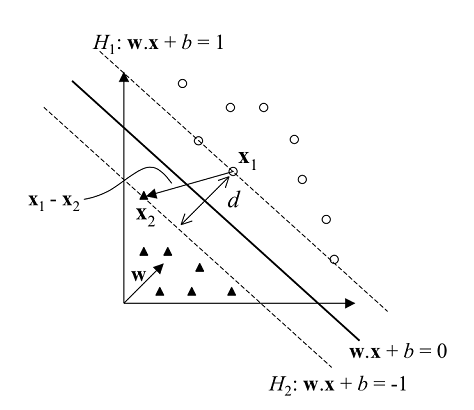
\includegraphics[scale=0.5]{./figuras/margem_svm.png}
	\caption{Hiperplano separador representado pela linha no meio e hiperplanos de apoio $H_{1}$ e $H_{2}$ representado pelas retas pontinhadas nas extremidades, assim com os vetores de suporte como $x_{1}$ e $x_{2}$ e a distância $d$ (Adaptado de \cite{Lorena2007}}
	\label{fig:margem_svm}
\end{figure}

Para maximizar a distância $d$, onde procura-se encontrar a distância que melhor separa os dados, podemos recorrer ao seguinte problema de otimização:

\begin{equation} \label{svm:E9}
\text{Minimizar}_{w,b}\  \frac{1}{2}\parallel w \parallel^{2}
\end{equation}

\begin{equation} \label{svm:E10}
\text{Sujeito às restrições: } y_{i}(w \cdot x_{i} + b) - 1 \geq 0, \ \ \forall i=1,...,n
\end{equation}

Note que a restrição impede que haja dados de treinamento entre as margens de separação das classes. Por isso o nome de SVM de margens rígidas.

O problema obtido é do tipo quadrático, para a resolução desse problema existem vários métodos que serão visto na Seção \ref{spq}. Para a resolução de problemas dessa categoria é necessário a substituição da formulação do problema para uma formulação Lagrangiana. Isto é feito porque a restrição \ref{svm:E10} será substituída por restrições na forma de multiplicadores de Lagrange, que trazem facilidades na resolução. Outro motivo, é que os dados de treinamento irão aparecer somente na forma de produto interno entre os dados, que irá ajudar no procedimento de generalização no caso não-linear(\ref{cap:svm:svm-nl}) \cite{Burges1998Support}. Transformando as Equações \ref{svm:E9} e \ref{svm:E10}, em uma função Lagrangiana obtemos:

\begin{equation} \label{svm:E11}
L(w,b,\alpha) = \frac{1}{2}\parallel w \parallel^2 - \sum_{i}^{n} \alpha_{i}(y_{i}(w \cdot x_{i} + b) - 1)
\end{equation}

Para minimizar a função Lagrangiana, é necessário maximizar as variáveis $\alpha_{i}$ e minimizar $w$ e $b$. Calculando o gradiente de $L$ em relação a $w$ e $b$ nos da as seguintes condições \cite{Burges1998Support}:

\begin{equation}\label{svm:E12}
w = \sum_{i = 1}^{n} \alpha_{i}y_{i}x_{i}
\end{equation}

\begin{equation}\label{svm:E13}
\sum_{i = 1}^{n} \alpha_{i}y_{i} = 0
\end{equation}

Substituindo as Equações \ref{svm:E12} e \ref{svm:E13} na Equação \ref{svm:E11} obtemos:

\begin{equation}\label{svm:E14}
\text{Maximizar}_{\alpha} \sum_{i = 1}^{n} \alpha_{i} - \frac{1}{2} \sum_{i,j = 1}^{n} \alpha_{i}\alpha_{j}y_{i}y_{j}(x_{i} \cdot x_{j})
\end{equation}

\begin{equation} \label{svm:E15}
\text{Sujeito às restrições:} 
\left\{\begin{matrix}
\alpha \geq 0, \  \forall i = 1,...,n \\ 
\sum_{i = 1}^{n} \alpha_{i}y_{i} = 0  &
\end{matrix}\right.
\end{equation}

Este tipo de formulação é conhecido como a forma dual, e a anterior (sem multiplicadores de Lagrange) como forma primal. 

Na solução dual para cada dado de treinamento temos um $\alpha_{i}$, e todos os dados onde $\alpha_{i} > 0$, são chamados de vetores de suporte, e estão localizados em um dos hiperplanos $H_{1}$ ou $H_{2}$. Os dados cujo o $\alpha_{i} = 0$, estão no mesmo lado de $H_{1}$ ou $H_{2}$, de tal forma que não viole a restrição imposta na Equação \ref{svm:E10}. Esses dados não participam do cálculo de $w$ (Equação\ref{svm:E12}). Para encontrar o valor de $b$, são feitos cálculos a partir do vetores de suporte (VT) conforme é mostrado na Equação \ref{svm:E16}.

\begin{equation} \label{svm:E16}
b = \frac{1}{n_{VT}} \sum_{x_{j} \in VT} \left(\frac{1}{y_{j}} - \sum_{x_{j} \in VT} \alpha_{i}y_{i}x_{i} \cdot x_{j} \right)
\end{equation}
onde $n_{VT}$ é o número de vetores de suporte.

Assim chegamos a função do classificador linear (Equação \ref{svm:E17}), está função representa o hiperplano que separa os dados com a margem, considerando aqueles com maior capacidade de generalização.

\begin{equation} \label{svm:E17}
f(x) = \left(\sum_{x_{i} \in VT} y_{i}\alpha_{i}x_{i} \cdot x + b \right)
\end{equation}

\subsection{SVM com margem suave}
Nas SVMs com a margem rígida é assumido que os dados são totalmente heterogêneos, com solução só para casos sem a presença de ruídos ou \textit{outliers}. Entretanto na prática é comum que os dados contenham ruídos e \textit{outliers}. Nesta seção veremos como contornar este obstaculo com a introdução das SVMs de margem suave. Isto é feito através da generalização do caso com margens rígidas, introduzindo um variável de folga $\xi_{i}, i= 1,...,l$, nas restrições impostas ao problema de otimização primal, que se tornam  \cite{Scholkopf2002}: 

\begin{equation} \label{svm:E18}
y_{i}(w \cdot x_{i} + b) \geq 1 - \xi_{i}, \  \xi_{i} \geq 0, \forall i =1,...,n
\end{equation}

Com a aplicação do $\xi_{i}$, as margens do classificador ficara suavizada, permitindo que dados permaneçam entre os hiperplanos $H_{1}$ e $H_{2}$, assim como erros de classificação.

Para que ocorra um erro é necessário que o erro exceda um limite. Este limite é a soma dos $\sum_{i} \xi_{i}$ que é um limite superior do número de erros de treinamento \cite{Burges1998Support}. Devemos modificar a função objetivo da Equação \ref{svm:E9} para conter o custo extra para erros, que fica:

\begin{equation}\label{svm:E19}
\text{Minimizar}_{w,b,\xi} \frac{1}{2}\parallel w \parallel^{2} + C \left( \sum_{i=1}^n \xi_{i}\right)
\end{equation}

A constante $C$ é um parâmetro definido pelo usuário e ela atua como um termo de regularização da complexidade do modelo em relação a margem de erros, um valor alto de $C$ significa uma alta penalidade para erros \cite{passerini04kernelmethods}

O problema de otimização gerado novamente é quadrático semelhante ao de margens rígidas, mas com as restrições da Equação \ref{svm:E18}, com os multiplicadores de Lagrange temos o seguinte problema dual:

\begin{equation}\label{svm:E20}
\text{Maximizar}_{\alpha} \sum_{i = 1}^{n} \alpha_{i} - \frac{1}{2} \sum_{i,j = 1}^{n} \alpha_{i}\alpha_{j}y_{i}y_{j}(x_{i} \cdot x_{j})
\end{equation}

\begin{equation} \label{svm:E21}
\text{Sujeito as restrições:} 
\left\{\begin{matrix}
0 \leq \alpha \leq C, \  \forall i = 1,...,n \\ 
\sum_{i = 1}^{n} \alpha_{i}y_{i} = 0  &
\end{matrix}\right.
\end{equation}

A única diferença em relação ao caso anterior é que o $\alpha_{i}$ tem um limite superior de $C$. Para uma solução ótima
do problema dual, encontramos o valor das variáveis $\xi_{i}$ pela seguinte equação:

\begin{equation}\label{svm:E22}
\xi_{i} = max \left\lbrace 0,1 - y_{i} \sum_{j=1}^{n}y_{j}\alpha_{j}x_{j} \cdot x_{i} + b \right\rbrace
\end{equation}

Para encontrar $b$ como no caso rígido ele provém de $\alpha$ e de condições KKT( Karush-Kuhn-Tucker) representadas nas Equações \ref{svm:E23} e \ref{svm:E24} \cite{Scholkopf2002}.

\begin{equation} \label{svm:E23}
\alpha_{i}(y_{i}(w \cdot x_{i} + b) - 1 + \xi_{i}) = 0
\end{equation}

\begin{equation} \label{svm:E24}
(C - \alpha_{i})\xi_{i} = 0
\end{equation}

Pelas condições de KKT das Equações \ref{svm:E23} e \ref{svm:E24}, podemos definir os vetores de suporte que diferente do caso rígido pode assumir três tipos distintos \cite{Scholkopf2002}:
\begin{itemize}
\item $\alpha_{i} = 0$ e $\xi_{i} = 0$. Então o dado $x_{i}$ é corretamente classificado e encontra-se fora das margens.
\item $0 < \alpha_{i} < C$ e $\xi_{i} = 0$. Então o dado $x_{i}$ é um vetor de suporte que encontra-se entre as margens, também denominado de livres.
\item $\alpha = C$. Então temos três casos: o dado $x_{i}$ é um erro se e $\xi_{i} > 1$; $x_{i}$ é classificado corretamente mas entre as margens,se $0 < \xi_{i} \leq 1$; ou $x_{i}$ fica sobre as margens, se $\xi_{i} = 0$.
\end{itemize}

\begin{figure}[htb]
	\centering
	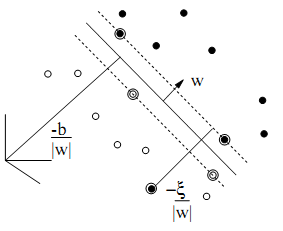
\includegraphics[scale=0.9]{./figuras/margem_svm_suave.png}
	\caption{Exemplo de classificador SVM com margens suaves (Adaptado de \cite{Burges1998Support}}
	\label{fig:margem_svm_suave}
\end{figure}

Na Figura \ref{fig:margem_svm_suave} os dados circulados na linha tracejada são os vetores de suporte livres. O dado de cor preta que está do outro lado do hiperplano é considerado um erro. 

\section{SVMs não-linear}\label{cap:svm:svm-nl}

As SVMs lineares descritas anteriormente são eficazes na classificação de dados que podem ser separados linearmente por um hiperplano. Porém para os dados de treinamento que não são separáveis linearmente, as SVMs não conseguem obter resultados satisfatórios. Para contornar esse problema será introduzido as SVMs não-linear. Para o caso não-linear é necessário a transformação dos dados de seu espaço original $x$ para um novo espaço de maior dimensão $\Phi(x)$ onde é possível separar os dados linearmente. Então é aplicado a metodologia apresentada para o caso linear, para encontrar o hiperplano separador nos dados transformados classificando-os corretamente \cite{Steinbach2005}. As Figuras \ref{fig:1d-to-2d-svm} e \ref{fig:2d-to-3d}, são dois exemplos de dados que em seus espaços originais não é possível separa-los com um hiperplano mas quando transformamos o espaço para outra dimensão, é possível fazer a separação dos dados.

\begin{figure}[htb]
	\centering
	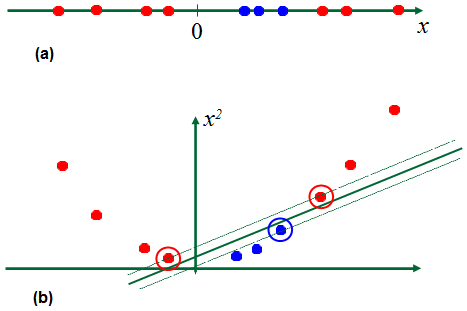
\includegraphics[scale=0.5]{./figuras/1d-to-2d-svm.png}
	\caption{(a) Conjunto de dados que não podem ser separados no espaço original; (b) Transformação do espaço para que seja possível a separação dos dados}
	\label{fig:1d-to-2d-svm}
\end{figure}

\begin{figure}[htb]
	\centering
	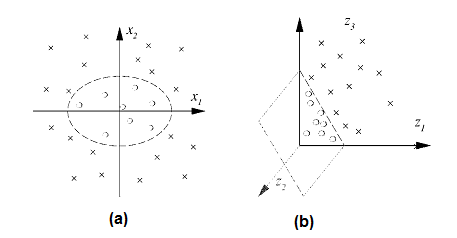
\includegraphics[scale=0.8]{./figuras/2d-to-3d.png}
	\caption{(a) Conjunto dados não linear; (b) Separação dos dados em (a) com a transformação do espaço (Adaptado de \cite{Muller2001})}
	\label{fig:2d-to-3d}
\end{figure}

No processo de transformação dos dados $\Phi: \Re^{d} \rightarrow \aleph$ é um mapeamento, onde $\Re^{d}$ é o espaço de entradas e $\aleph$ é o novo espaço com dimensão maior, também conhecido com espaço de características. Nosso objetivo é escolher corretamente $\Phi$, para que o conjunto de treinamento seja mapeado em $\aleph$ onde a fronteira de decisão é linear.

\cite{Muller2001} apresenta um exemplo simples desse mapeamento, que é a transformação feita na Figura \ref{fig:2d-to-3d}, onde os dados em $\Re^2$ são mapeados para a $\Re^3$. Para fazer o mapeamento $\Phi:\Re^2 \rightarrow \Re^3$ é utilizado a Equação \ref{svm:E25}, aplicando a equação o conjunto de dados em $\Re^2$ transforma-se em dados linearmente separáveis em $\Re^3$. Em $\Re^3$ é possível encontrar um hiperplano que separa os dados (Equação \ref{svm:26}). Embora a equação do hiperplano seja linear em $\Re^3$ ela não é linear em $\Re^2$.

\begin{equation}\label{svm:E25}
\Phi(x) = \Phi(x_{1},x_{2}) = \left(x_{1}^2,\sqrt{2x_{1}}x_{2},x_{2}^2\right)
\end{equation}

\begin{equation} \label{svm:E26}
f(x) = w \cdot \Phi(x) + b = w_{1}x_{1}^2 + w_{2} \sqrt{2x_{1}}x_{2} + w_{3}x_{2}^2 + b = 0
\end{equation}

A separação dos dados na nova dimensão é feita com a SVM de margens suáveis, para permitir ruídos e \textit{outliers}. Coma a adição do mapeamento de dados $\Phi$ a função de otimização da Equação \ref{svm:E20} fica conforme representado na Equação \ref{svm:E27}. As restrições são as mesmas da SVM linear de margens suáveis (Equação \ref{svm:E21}). E a função de decisão será na forma apresentada na Equação

\begin{equation} \label{svm:E27}
\begin{matrix}
\text{Maximizar}_{\alpha} \sum_{i = 1}^{n} \alpha_{i} - \frac{1}{2} \sum_{i,j = 1}^{n} \alpha_{i}\alpha_{j}y_{i}y_{j}(\Phi(x_{i}) \cdot \Phi(x_{j})) \\ 
0 \leq \alpha \leq C,\  \forall i = 1,...,n \\
\sum_{i = 1}^{n} \alpha_{i}y_{i} = 0
\end{matrix}.
\end{equation}



\begin{equation} \label{svm:E28}
f(x) = \sum_{x_{i} \in SV}\alpha_{i}y_{i}\Phi(x_{i}) \cdot \Phi(x) + b
\end{equation}

Nota-se pela Equação \ref{svm:E28} que os dados aparecem na forma de produtos interno, $\Phi(x_{i} \cdot \Phi_{j})$, e que a única informação necessária para o mapeamento é como realizar o produto interno. Este tipo calculo é muito custoso \cite{Scholkopf2002}, mas ele pode ser reduzido para uma função \textit{Kernel} $K$ tal que:

\begin{equation} \label{svm:E29}
K(x_{i},x_{j}) = \Phi(x_{i}) \cdot \Phi(x_{j}))
\end{equation} 
 
Assim só usamos $k$ no algoritmo de treinamento, sem a necessidade de explicitar ou saber o que é $\Phi$ \cite{Burges1998Support}.

As funções kernel utilizadas nas SVMs seguem as condições estabelecidas pelo teorema de Mercer \cite{Burges1998Support}. É utilizado este teorema para que seja garantida a convexidade do problema de otimização (Equação \ref{svm:E27}) e para que os mapeamentos representados pelo kernel possibilite o cálculo de produtos escalares (Equação \ref{svm:E29}).

Não existe uma função \textit{kernel} melhor do as outras, o desempenho depende do tipo de dados de cada aplicação. A seguir serão apresentados as funções \textit{kernel} mais comum, que são:
\begin{itemize}
\item Produto interno:
\begin{equation}
K(x_{i},x_{j}) = x_{i}^T \cdot x_{j}
\end{equation}

\item Polinomial Homogêneo:
\begin{equation}
K(x_{i},x_{j}) = (x_{i}^T \cdot x_{j})^p
\end{equation}
onde:
$p$ é o grau do polinômio

\item Polinomial Não Homogêneo:
\begin{equation}
K(x_{i},x_{j}) = (x_{i}^T + c)^p
\end{equation}
onde:
$p$ é o grau do polinômio
$c$ é uma constante

\item Sigmoidal:
\begin{equation}
K(x_{i},x_{j}) = tanh(\kappa x_{i} \cdot x_{j} + c)
\end{equation}
onde:
$\kappa$ é um coeficiente
$c$ é uma constante

\item Gaussiano:
\begin{equation}
K(x_{i},x_{j}) = e^{\frac{\mid x_{i} - x_{j} \mid}{2\sigma^2} }
\end{equation}
onde:
$\sigma$ é um parâmetro
\end{itemize}

\section{Soluções da programação quadrática do SVM}\label{spq}

A modelagem do SVM envolve o problema de programação quadrática apresentado na Seção \ref{Teot}. Foram propostos vários métodos para sua resolução. Entretanto devido ao grande tamanho das entradas, a forma quadrática (Equação \ref{svm:E27}) que aparece não pode ser resolvida facilmente pelas técnicas padrão de programação quadrática. Está seção revisará os principais métodos. Iniciaremos com o método Chunking (Subseção \ref{spqS1}), na sequência o método de Decomposição (Subseção \ref{spqS2}), e finalmente (Subseção \ref{spqS3}) o \textit{Sequential Minimal Optimization} (SMO), neste será dado maior atenção, por ele ser de fácil implementação, de baixa complexidade e obter resultados satisfatórios e muitas vezes superiores que os demais métodos.

\subsection{Chunking} \label{spqS1}

Este método trabalha apenas com uma parte dos dados e utilizar somente vetores de suporte para encontrar a solução. Ele começa com uma parte arbitrária dos dados chamada '\textit{chunk}', então treina a SVM usando um otimizador quadrático qualquer. Do subconjunto treinado é mantido apenas os vetores de suporte, os demais são todos descartados, e é testado a hipótese encontrada com os vetores de suporte no restante dos dados. Os $M$ piores dados de treinamento, que violam as condições de KKT (onde $M$ é um parâmetro), são adicionados no conjunto de vetores de suporte encontrados no passo anterior para formar um novo '\textit{chunk}'. Se existe um numero menor que $M$ de exemplos que violam KKT, todos os dados que violam são adicionados ao conjunto. As iterações continuam até um critério de parada ser atingido, este critério, por exemplo, pode ser um limite no número de iterações ou até que todos os dados forem processados. Este método possui algumas falhas. A primeira é que o conjunto de vetores de suporte são armazenados na memória se esse conjunto for muito grande poderá ocorrer problemas por falta de memória. Outro problema que também envolve o tamanho do conjunto de vetores, é a falha de alguns otimizadores quadrático, devido a o conjunto ser extenso \cite{Cristianini2000,Platt1999}.

\subsection{Decomposição} \label{spqS2}

Semelhante ao método de \textit{Chunking}, o método de decomposição também reparte o problema quadrático em vários subproblemas. A principal diferença entre eles, é que no método de decomposição o subconjunto tem um número fixado de elementos. Então para cada item adicionado ao conjunto outro tem que ser removido. Neste algoritmo não será identificado todos os vetores de suporte, mas sim aqueles que otimizam o problema globalmente. Para isto os pontos incluídos no conjunto de trabalho são os que violam as condição KKT. Assim com no anterior a computação do problema quadrático é feita externamente.

\subsection{Sequential Minimal Optimization} \label{spqS3}

O \textit{Sequential Minimal Optimization} (SMO) é um algoritmo que resolve o problema quadrático de forma eficiente, rápida e sem muitos gastos de memória, uma vez que não é necessário guardar um conjunto de vetores de suporte na memória. Este algoritmo foi introduzido por \cite{Platt1999}. Ele tem algumas semelhanças com os algoritmos descritos nas seções anteriores, por exemplo ele também trabalha com subproblemas, mas contendo apenas dois pontos em cada iteração. O ponto chave deste algoritmo que o faz obter resultados melhores que os demais é que quando o conjunto de trabalho tem apenas dois elementos é possível resolver o problema analiticamente, eliminando a necessidade de usar um otimizador quadráticos como parte do algoritmo (pacote de terceiros). 

Destacam-se três componentes no SMO: o método analítico para resolver os dois pontos, uma heurística para escolher qual ponto otimizar, e um método para calcular o bias $b$. Estes três componeste serão discutidos a seguir.

\subsubsection{Solução analítica para dois pontos}

Vamos assumir que os pontos escolhidos para a solução analítica são $\alpha_{1} \ e \  \alpha_{2}$, que são multiplicadores. Primeiramente o SMO computa as restrições nos multiplicadores e então resolve para a restrição máxima. As restrições são representadas na Figura \ref{fig:smo-restric}.

\begin{figure}[htb]
	\centering
	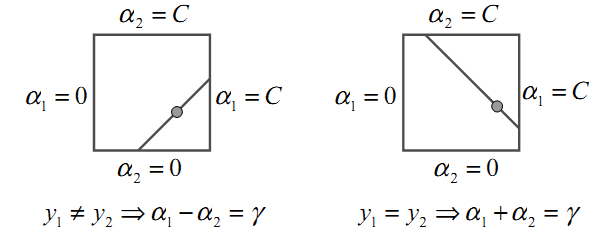
\includegraphics[scale=0.7]{./figuras/smo-restric.png}
	\caption{Restrições nos dois multiplicadores}
	\label{fig:smo-restric}
\end{figure}

O limite de restrição em \ref{svm:E27} ($0 \leq \alpha_{i} \leq C$) faz com que os multiplicadores de Lagrange repouse em uma caixa, enquanto que a equação linear de \ref{svm:E27} ($\sum_{i}^l y_{i}\alpha_{i} = 0$), faz os multiplicadores repousarem em uma linha diagonal. A restrição máxima da função objetivo irá repousar em uma reta diagonal \cite{Platt1999}. O problema de uma dimensão resultante da restrição da função objetivo pode ser solucionado analiticamente.

O algoritmo primeiramente computa $\alpha_{2}^{novo}$ e sucessivamente usa-o para obter $\alpha_{1}^{novo}$. A restrição $0 \leq \alpha_{i} \leq C$ juntamente com a restrição linear, prove uma restrição mais rígida nos possíveis valores para $\alpha_{2}^{novo}$.

\begin{equation}\label{spq:E1}
L \leq \alpha_{2}^{novo} \leq H
\end{equation}
onde:
\begin{equation}\label{spq:E2}
L = max(0, \alpha_{2}^{antigo} - \alpha_{1}^{antigo}),\ \ \ \ H = min(C, C - \alpha_{1}^{antigo} + \alpha_{2}^{antigo}),
\end{equation}
se $y_{1} \neq y_{2}$, e

\begin{equation}\label{spq:E3}
L = max(0, \alpha_{1}^{antigo} + \alpha_{2}^{antigo} - C),\ \ \ \ H = min(C, \alpha_{1}^{antigo} + \alpha_{2}^{antigo}),
\end{equation}
se $y_{1} = y_{2}$.

Para encontrar o máximo da função objetivo \ref{svm:E27}, utilizaremos o erro definido na Equação \ref{spq:E4} , que é a diferença entre a função de saída e do valor desejado.

\begin{equation}\label{spq:E4}
E_{i} = f(x) - y_{i} = \left(\sum_{j=1}^{j} \alpha_{j}y_{j}K(x_{j},x_{i}) + b \right) - y_{i},i=1,2
\end{equation}

Também é necessário um valor adicional que é a derivada da função objetivo ao longo da linha diagonal, que pode ser expressada por $k$, definido por:

\begin{equation}\label{spq:E5}
k = K(x_{1},x_{1})+K(x_{2},x_{2}) - 2K(x_{1},x_{2}) = \parallel \Phi(x_{1}) - \Phi(x_{2}) \parallel^2,
\end{equation}

O valor máximo da função objetivo, é obtido com:

\begin{equation}
\alpha_{2}^{novo} = 
\left\{\begin{matrix}
H, & se & \alpha_{2}^{aux} > H, \\ 
\alpha_{2}^{aux}, & se & L \leq \alpha_{2}^{aux} \leq H, \\
L, & se & \alpha_{2}^{aux} < L.
\end{matrix}\right.
\end{equation}

$\alpha_{2}^{aux}$ é limitado por $L \leq \alpha_{2}^{aux} \leq H$, dado por:
\begin{equation}
\alpha_{2}^{aux} = \alpha_{2}^{antigo} + \frac{y_{2}(E_{1} - E_{2})}{k}
\end{equation}

O valor de $\alpha_{1}^{novo}$ é obtido através de $\alpha_{2}^{novo}$, dado por:

\begin{equation}
\alpha_{1}^{novo} = \alpha_{1}^{antigo} + y_{1}y_{2}(\alpha_{2}^{antigo} - \alpha_{2}^{novo}).
\end{equation}

As formulações acima faz parte de um teorema e a prova pode ser conferida em \cite{Cristianini2000}.

\subsubsection{Seleção das Heurísticas}

O SMO utiliza duas heurísticas para a seleção de dois pontos ativos para garantir que a função objetivo aproveite um grande aumento de sua otimização. Existem duas heurísticas para a escolha do primeiro e do segundo ponto.

Na primeira heurística o primeiro ponto $x_{1}$ é escolhido entre os pontos que violam as condições de KKT. Um laço externo no algoritmo percorre o conjunto de treinamento a procura de pontos que violam as condições de KKT e seleciona um para atualizar. Quando um ponto é encontrado a segunda heurística é chamada para selecionar o segundo ponto, e os valores de seu respectivo multiplicador é atualizado. A segunda heurística deve escolher o segundo ponto $x_{2}$, de tal maneira que atualizando o par $\alpha_{i},\alpha_{2}$ cause uma grande mudança, que resulta em um aumento significativo da função objetivo dual \cite{Cristianini2000}. 

Para encontrar o segundo ponto sem muitos cálculos  de maneira que este ponto seja uma boa escolha, uma rápida heurística é escolhida para encontrar $x_{2}$, maximizando o valor $\mid E_{1} - E_{2} \mid$. Se $E_{1}$ é positivo, SMO escolhe um exemplo $x_{2}$ com menor erro $E_{2}$, enquanto se $E_{1}$ é negativo, SMO maximiza o erro $E_{2}$ \cite{Cristianini2000}. 

O valor $b$ é recalculado depois de cada iteração, onde as condições de KKT são satisfeitas para ambos pontos. O valor $b_{1}$ é valido quando  $\alpha_{1}^{novo}$ não esta no limiar, isto força a saída do SVM ser $y_{1}$ quando a entrada for $x_{1}$:

\begin{equation}
b_{1} = E_{1} + y_{1}(\alpha_{1}^{novo} - \alpha_{1}^{antigo})k(x_{1},x_{1})+y_{2}(\alpha_{2}^{novo} - \alpha_{2}^{antigo})k(x_{1},x_{2})+b^{antigo}
\end{equation}

O valor $b_{2}$ é valido quando  $\alpha_{2}^{novo}$ não esta no limiar, isto força a saída do SVM ser $y_{2}$ quando a entrada for $x_{2}$:

\begin{equation}
b_{2} = E_{2} + y_{1}(\alpha_{1}^{novo} - \alpha_{1}^{antigo})k(x_{1},x_{1})+y_{2}(\alpha_{2}^{novo} - \alpha_{2}^{antigo})k(x_{2},x_{2})+b^{antigo}
\end{equation}

Quando $b_{1}$ e $b_{2}$ são validos, eles são iguais. Quando ambos multiplicadores de Lagrange novos estão no limite e se $L$ não é igual a $H$, então o intervalo entre $b_{1}$ e $b_{2}$ são todos limiar que estão consistentes com as condições de KKT. Nesse caso o SMO escolhe o limiar intermediário entre $b_{1}$ e $b_{2}$ \cite{Platt1999}. 

\cite{Platt1999} apresenta um pseudocódigo do algoritmo de classificação SMO, detalhando os principais pontos necessários para implementação do SMO.